
\definecolor{ornl_green}{RGB}{42, 100, 51}
\definecolor{snl_blue}{RGB}{75, 165, 226}
\definecolor{cea_red}{RGB}{204, 43, 40}
% \definecolor{github_black}{RGB}{255, 255, 255}
\definecolor{hpsf_purple}{RGB}{110, 39, 107}
\definecolor{nersc_blue}{RGB}{14, 43, 80}


\begin{frame}[fragile]{Founding of CI-WG}
  \begin{center}
\textbf{Kokkos founded a working group for continuous integration}
\vspace{1cm}
  \end{center}

    Objectives
    \begin{itemize}
      \item{Redistribute testing to more institutions}
      \item{Increase coverage}
      \item{Diversify knowledge to increase robustnes}
    \end{itemize}

\end{frame}

\begin{frame}[fragile]{CI coverage of backends}

  \begin{center}
    \begin{minipage}{.45\textwidth}
    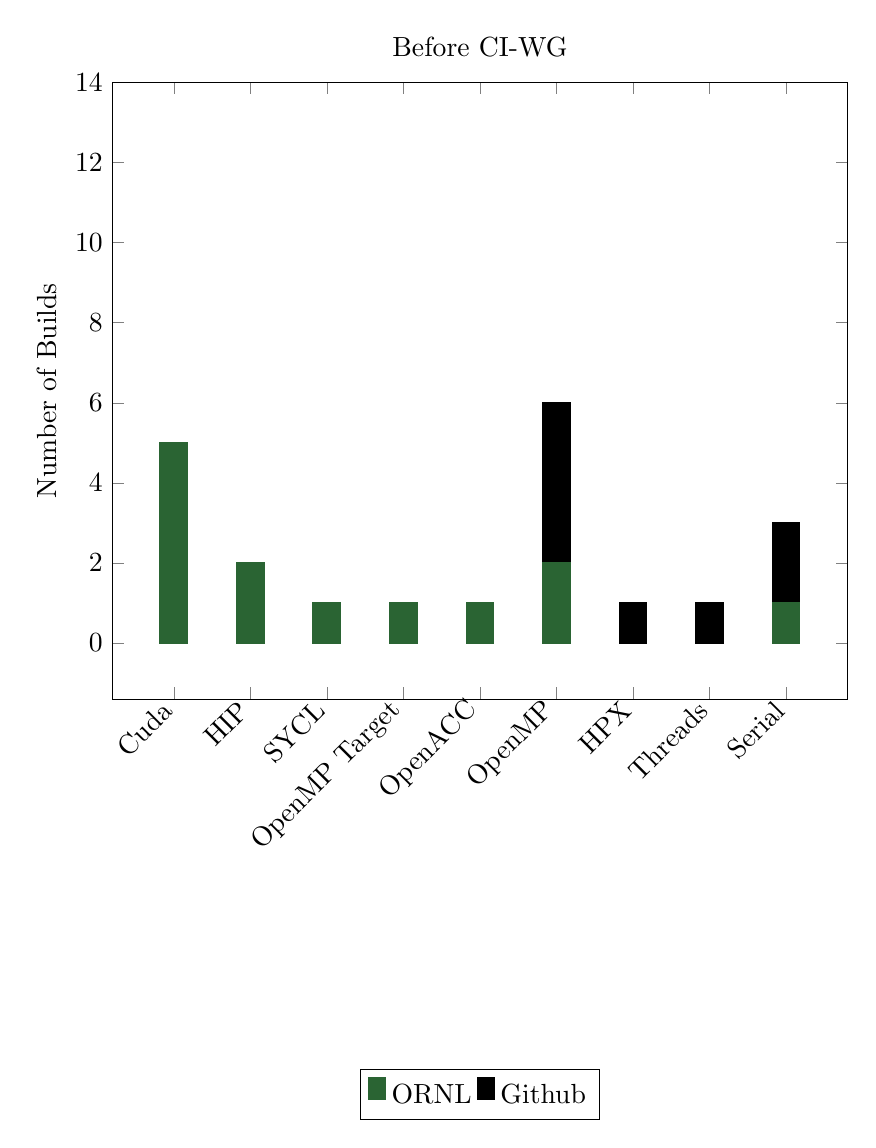
\begin{tikzpicture}
  \begin{axis}[
    title={Before CI-WG},
    ybar stacked,
    ymax=14,
    symbolic x coords={Cuda, HIP, SYCL, OpenMP Target, OpenACC, OpenMP, HPX, Threads, Serial},
    xticklabel style={rotate=45,anchor=east},
    xtick=data,
    width=0.9\textwidth,
    legend style={at={(0.5,-0.60)},
      anchor=north,legend columns=-1},
    ylabel=Number of Builds]
  \addplot+[ybar,color=ornl_green] plot coordinates {(Cuda,5) (HIP,2) (SYCL,1) (OpenMP Target,1) (OpenACC,1) (OpenMP,2) (HPX,0) (Threads,0) (Serial,1)};
  \addplot+[ybar,color=black] plot coordinates {(Cuda,0) (HIP,0) (SYCL,0) (OpenMP Target,0) (OpenACC,0) (OpenMP,4) (HPX,1) (Threads,1) (Serial,2)};
  % \addplot+[ybar,color=snl_blue] plot coordinates {(Cuda,2) (HIP,2) (SYCL,2) (OpenMP Target,0) (OpenACC,0) (OpenMP,2) (HPX,0) (Threads,2) (Serial,0)};
  % \addplot+[ybar,color=cea_red] plot coordinates {(Cuda,0) (HIP,0) (SYCL,0) (OpenMP Target,0) (OpenACC,0) (OpenMP,0) (HPX,0) (Threads,0) (Serial,0)};
  % \addplot+[ybar,color=hpsf_purple] plot coordinates {(Cuda,0) (HIP,0) (SYCL,0) (OpenMP Target,0) (OpenACC,0) (OpenMP,0) (HPX,0) (Threads,0) (Serial,0)};
  % \addplot+[ybar,color=nersc_blue] plot coordinates {(Cuda,0) (HIP,0) (SYCL,0) (OpenMP Target,0) (OpenACC,0) (OpenMP,0) (HPX,0) (Threads,0) (Serial,0)};
  \legend{\strut ORNL, \strut Github}
  % \legend{\strut ORNL, \strut SNL, \strut CEA, \strut Github, \strut HPSF, \strut NERSC}
  \end{axis}
\end{tikzpicture}
\end{minipage}
\begin{minipage}{.45\textwidth}
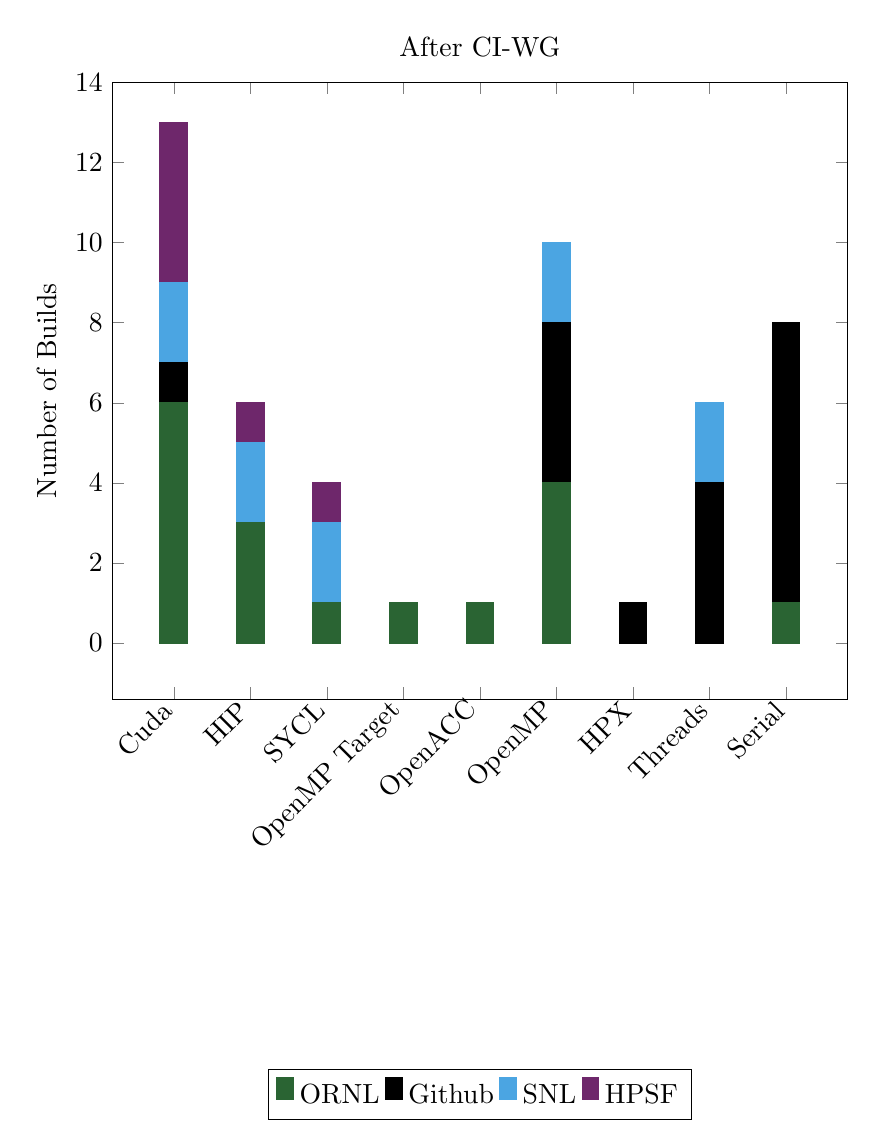
\begin{tikzpicture}
  \begin{axis}[
    title={After CI-WG},
    ybar stacked,
    ymax=14,
    symbolic x coords={Cuda, HIP, SYCL, OpenMP Target, OpenACC, OpenMP, HPX, Threads, Serial},
    xticklabel style={rotate=45,anchor=east},
    xtick=data,
    width=0.9\textwidth,
    legend style={at={(0.5,-0.60)},
      anchor=north,legend columns=-1},
    ylabel=Number of Builds]
  \addplot+[ybar,color=ornl_green] plot coordinates {(Cuda,6) (HIP,3) (SYCL,1) (OpenMP Target,1) (OpenACC,1) (OpenMP,4) (HPX,0) (Threads,0) (Serial,1)};
  \addplot+[ybar,color=black] plot coordinates {(Cuda,1) (HIP,0) (SYCL,0) (OpenMP Target,0) (OpenACC,0) (OpenMP,4) (HPX,1) (Threads,4) (Serial,7)};
  \addplot+[ybar,color=snl_blue] plot coordinates {(Cuda,2) (HIP,2) (SYCL,2) (OpenMP Target,0) (OpenACC,0) (OpenMP,2) (HPX,0) (Threads,2) (Serial,0)};
  % \addplot+[ybar,color=cea_red] plot coordinates {(Cuda,0) (HIP,0) (SYCL,0) (OpenMP Target,0) (OpenACC,0) (OpenMP,0) (HPX,0) (Threads,0) (Serial,0)};
  \addplot+[ybar,color=hpsf_purple] plot coordinates {(Cuda,4) (HIP,1) (SYCL,1) (OpenMP Target,0) (OpenACC,0) (OpenMP,0) (HPX,0) (Threads,0) (Serial,0)};
  % \addplot+[ybar,color=nersc_blue] plot coordinates {(Cuda,0) (HIP,0) (SYCL,0) (OpenMP Target,0) (OpenACC,0) (OpenMP,0) (HPX,0) (Threads,0) (Serial,0)};
  % \legend{\strut ORNL, \strut SNL, \strut Github}
  \legend{\strut ORNL, \strut Github, \strut SNL, \strut HPSF}
  \end{axis}
\end{tikzpicture}
\end{minipage}
  \end{center}

\end{frame}
